\documentclass[t]{beamer}
\usetheme[english]{KIT}

\usepackage{amssymb} %% For \backprime
\usepackage{multicol}

%\usepackage{mathpartir}
\usepackage{graphicx}

\usepackage{tikz}
\usetikzlibrary{arrows.meta,positioning,calc}

\usepackage[T1]{fontenc}
\usepackage{babel}
\usepackage{booktabs}
\usepackage[normalem]{ulem}
\usepackage{fontspec}
\setmonofont[Scale=MatchLowercase]{Iosevka}
%\newfontfamily\lc[Scale=MatchLowercase]{Iosevka SS09}

\usepackage{minted}
\definecolor{codebg}{rgb}{0.95,0.95,0.95}
\setminted{bgcolor=codebg,breaklines}
\usemintedstyle{tango}
\newmintinline[lean]{lean}{bgcolor=white}
\newminted{lean}{fontsize=\footnotesize}

\usepackage{newunicodechar}
\newfontfamily{\freeserif}{DejaVu Sans}
\newunicodechar{ℕ}{\freeserif{ℕ}}
\newunicodechar{ℝ}{\freeserif{ℝ}}
\newunicodechar{ₐ}{\freeserif{ₐ}}
%\newunicodechar{₁}{\freeserif{₁}}
%\newunicodechar{∈}{\freeserif{∈}}
\newunicodechar{𝓞}{\ensuremath{\mathcal{O}}}
\newunicodechar{∉}{\freeserif{∉}}
%\newunicodechar{Π}{\freeserif{Π}}
%\newunicodechar{→}{\freeserif{→}}
\newunicodechar{⦃}{\freeserif{⦃}}
\newunicodechar{⦄}{\freeserif{⦄}}
%\newunicodechar{∧}{\freeserif{∧}}
%\newunicodechar{∨}{\freeserif{∨}}
%\newunicodechar{⊢}{\freeserif{⊢}}
\newunicodechar{⊑}{\freeserif{⊑}}
\newunicodechar{ₚ}{\freeserif{ₚ}}
\newunicodechar{∘}{\freeserif{∘}}
\newunicodechar{ₗ}{\freeserif{ₗ}}
\newunicodechar{∪}{\freeserif{∪}}
\newunicodechar{⋃}{\freeserif{⋃}}
\newunicodechar{𝓸}{\ensuremath{o}}
\newunicodechar{⊆}{\freeserif{⊆}}
\newunicodechar{≼}{\freeserif{≼}}
\newunicodechar{≃}{\freeserif{≃}}

% https://github.com/gpoore/minted/issues/220
\AtBeginEnvironment{snugshade*}{\vspace{-0.4\FrameSep}}
%\AfterEndEnvironment{snugshade*}{\vspace{-0.8\FrameSep}}

% https://tex.stackexchange.com/questions/343494/minted-red-box-around-greek-characters
\makeatletter
\AtBeginEnvironment{minted}{\dontdofcolorbox}
\def\dontdofcolorbox{\renewcommand\fcolorbox[4][]{##4}}
\makeatother

\title{Lean 4: State of the ⋃}

\author[Ullrich]{Sebastian Ullrich}
\subtitle{\insertauthor}
\institute[IPD Snelting]{Programming paradigms group - IPD Snelting}
\date{2020/01/09}
\makeatletter
\sbox{\KIT@titimg}{
  \hspace{0.08\titleimagewd}
    \raisebox{0.1\titleimageht}{
      
\includegraphics[height=0.8\titleimageht]{logo}
    }
}

\newcommand{\kit}[1]{\textcolor{KITgreen}{#1}}

\begin{document}
\begin{frame}
  \maketitle
\end{frame}

\begin{frame}{A brief history of Lean}
  \begin{itemize}
  \item Lean 0.1 (2014)
  \item Lean 2 (2015)
    \begin{itemize}
    \item first official release
    \item fixed tactic language
    \end{itemize}
  \item Lean 3 (2017)
    \begin{itemize}
    \item make Lean a \kit{meta-programming} language: build tactics in Lean
    \item backed by a bytecode interpreter
    \end{itemize}
  \item Lean 4 (201X)
    \begin{itemize}
    \item make Lean a \kit{general-purpose} language: native back end, FFI, ...
    \item reimplement Lean in Lean
    \end{itemize}
  \end{itemize}
  \visible<2>{
    \centering{\Huge{X $\ge 10$}}
  }
\end{frame}

\begin{frame}{The Lean dream team}
  \begin{itemize}
  \item Leonardo de Moura: everything, really
  \item Sebastian Ullrich: macros, interpreter
  \item<2-> Daniel Selsam: new typeclass resolution
  \item<3-> Simon Hudon: language server
  \end{itemize}
\end{frame}

\tikzset{
  invisible/.style={opacity=0},
  visible on/.style={alt={#1{}{invisible}}},
  alt/.code args={<#1>#2#3}{%
    \alt<#1>{\pgfkeysalso{#2}}{\pgfkeysalso{#3}} % \pgfkeysalso doesn't change the path
  },
}

\newcommand<>{\lol}[3]{
  \fill[#1!20] (path picture bounding box.north west)rectangle (path picture bounding box.south east);
  \alt#4{\fill[#1!50] (path picture bounding box.north west)rectangle ($(path picture bounding box.south west)!#3!(path picture bounding box.south east)$);}
  {\fill[#1!50] (path picture bounding box.north west)rectangle ($(path picture bounding box.south west)!#2!(path picture bounding box.south east)$);}
  }

\begin{frame}[fragile]
  \only<1>{\frametitle{Lean 4 progress: Jan 2019}}
  \only<2>{\frametitle{Lean 4 progress: Jun 2019}}
  \only<3>{\frametitle{Lean 4 progress: Dec 2019}}
  \only<4>{\frametitle{Lean 4 progress: Jan 2020}}
  \begin{center}
    \begin{tikzpicture}[>=stealth, thick, nodes={rounded corners, minimum height=2em}, level distance=12mm]
      \node[draw,fill=red!50][path picture={\lol<1>{red}{0}{0}}] (editor) {editor}
        child[<->] {
          node[draw,fill=blue!50][path picture={\lol<1>{green}{0}{0}}] {language server}
          child[->] {
            node[draw,fill=blue!50][path picture={\lol<2->{green}{0.8}{1}}] (parser) {parser}
            child {
              node[draw,fill=blue!50] [path picture={\lol<4->{green}{0.1}{0.5}}] (elab) {elaborator}
              child[->] {
                node[draw,fill=blue!50][path picture={\lol<1>{blue}{1}{1}}] {kernel}
              }
              child[->] {
                node[draw,fill=blue!50][path picture={
                  \lol<1>{blue}{0.8}{0.8}
                  \only<2->{
                    \fill[blue!50,sharp corners] (path picture bounding box.north west)rectangle ($(path picture bounding box.north east)!0.7!(path picture bounding box.south east)$);
                    \fill[green!50,sharp corners] ($(path picture bounding box.north west)!0.7!(path picture bounding box.south west)$)rectangle (path picture bounding box.south east);
                  }
}] (comp) {compiler}
              }
              edge from parent[draw=none]
            }
          }
        };
        \node[draw,right=of elab][path picture={\lol<4->{green}{0}{0.1}}] (tac) {tactic framework};
      \node[draw,fill=green!20,left=of elab][path picture={
        \only<3->{
        \fill[blue!50,sharp corners] (path picture bounding box.north west)rectangle ($(path picture bounding box.north east)!0.2!(path picture bounding box.south east)$);
        \fill[green!50,sharp corners] ($(path picture bounding box.north west)!0.2!(path picture bounding box.south west)$)rectangle (path picture bounding box.south east);
        }
}] (mod) {module system};
      \uncover<3->{
        \node[draw,above=3mm of mod][path picture={\lol<1>{green}{1}{1}}] {meta monad};
        \node[draw,below=3mm of mod][path picture={\lol<1>{green}{1}{1}}] {typeclass resolution};
      }
      \alt<1>{
        \node[draw,right=of parser][path picture={\lol<2->{green}{0.5}{1}}] (mac) {macro expander};
        \draw[->] (parser) to (mac);
        \draw[->] (mac) to (elab);
      }{
        \node[draw,right=of parser][path picture={\lol<2->{green}{0.7}{1}}] (mac) {macro hygiene};
        \draw[->] (parser) to (elab);
        \draw[-] (mac) to (elab);
      }
      \node[draw,below=3mm of comp][path picture={\lol<1>{blue}{0}{0}}] (ffi) {FFI};
      \draw[-] (comp) to (ffi);
      \only<3->{
        \node[draw,right=of ffi][path picture={\lol<1>{blue}{1}{1}}] (interp) {interpreter};
        \draw[-] (comp) to (interp);
      }
      \draw[->] (comp) to (tac);
      \draw[->] (tac) to (elab);
      \node[draw,left=35mm of editor,yshift=5mm,minimum height=5mm,minimum width=5mm][path picture={
        \fill[blue!20] (path picture bounding box.north west)rectangle (path picture bounding box.south east);
        \fill[blue!50] (path picture bounding box.north west)rectangle ($(path picture bounding box.south west)!0.5!(path picture bounding box.south east)$);
        }] (cpp) {};
        \node[right=1mm of cpp] {C++};
      \node[draw,below=1mm of cpp,minimum height=5mm,minimum width=5mm][path picture={
        \fill[green!20] (path picture bounding box.north west)rectangle (path picture bounding box.south east);
        \fill[green!50] (path picture bounding box.north west)rectangle ($(path picture bounding box.south west)!0.5!(path picture bounding box.south east)$);
        }] (lean) {};
        \node[right=1mm of lean] {Lean};
      \node[draw,below=1mm of lean,minimum height=5mm,minimum width=5mm][path picture={
        \fill[red!20] (path picture bounding box.north west)rectangle (path picture bounding box.south east);
        \fill[red!50] (path picture bounding box.north west)rectangle ($(path picture bounding box.south west)!0.5!(path picture bounding box.south east)$);
        }] (other) {};
        \node[right=1mm of other] {other};
    \end{tikzpicture}
  \end{center} 
\end{frame}

\begin{frame}[fragile]{Cosmetics}
  Minor syntax changes to make Lean a more consistent and pleasant language
  \bigskip

  \begin{itemize}
  \item<+-> naming convention: \texttt{TypeName},  \texttt{ModuleName}, \texttt{termName}
    \begin{itemize}
    \item<+-> lemma convention \verb!termName_property_of_assumption!?
    \end{itemize}
  \item<+-> consistent pattern syntax
    \vspace{-4mm}
    \begin{columns}
      \column{0.4\textwidth}
      \begin{leancode}
def hiThere : ...
| pat1, ... => ...
| ...
\end{leancode}
      \column{0.4\textwidth}
\begin{leancode}
match ... with
| pat1, ... => ...
| ...
\end{leancode}
    \end{columns}
  \item<+-> etc...
\begin{leancode}
fun x =>
  let y := 1;
  do a; b
\end{leancode}
  \end{itemize}
\end{frame}

\begin{frame}{Compiler}
  Ullrich and de Moura. \emph{Counting Immutable Beans: Reference Counting Optimized for Purely Functional Programming}. IFL'19.
  
  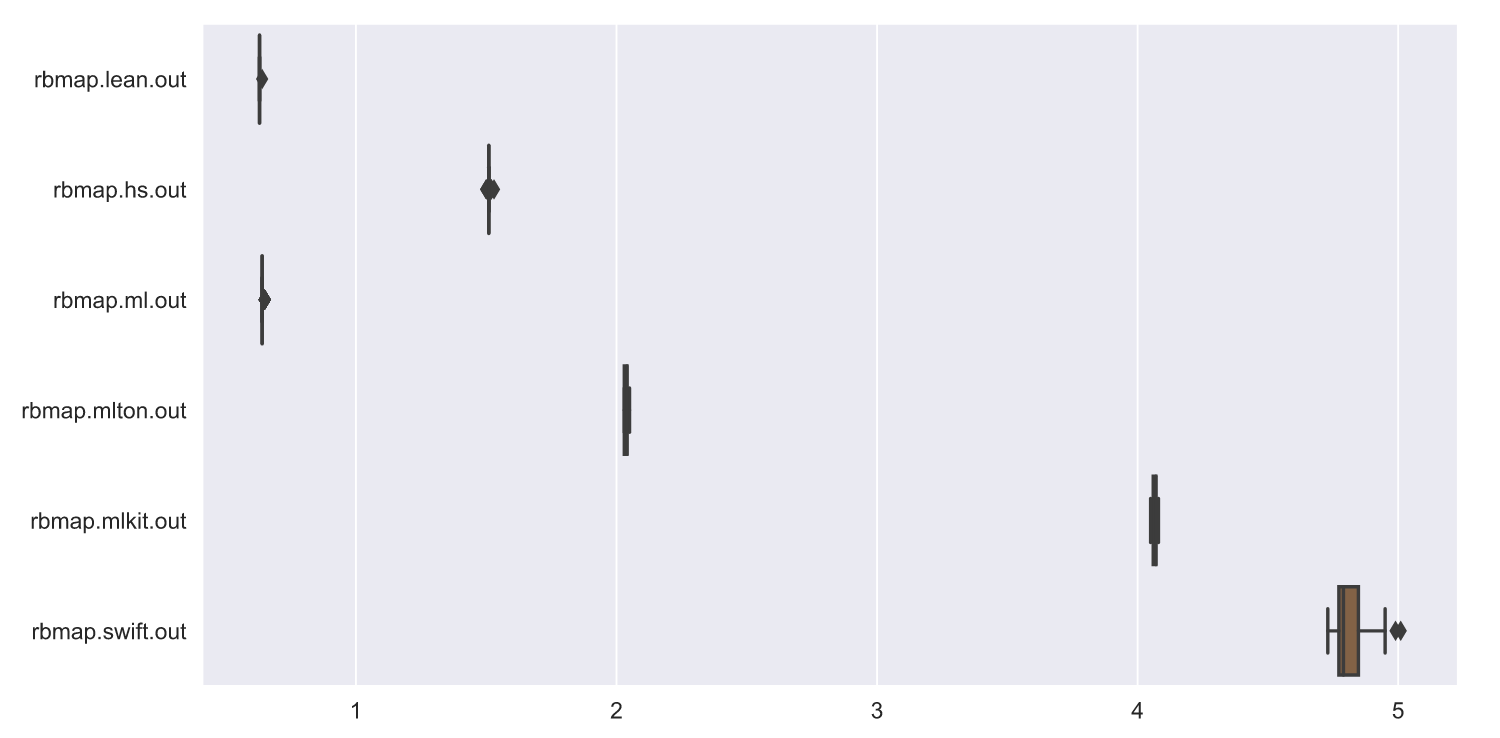
\includegraphics[width=\textwidth]{bench}
\end{frame}

\begin{frame}{New typeclass resolution}
  Performance issues with the old implementation:
  \begin{itemize}
  \item \emph{diamonds} can lead to exponential runtime
  \item cycles can lead to nontermination
  \end{itemize}
  \pause
  \bigskip

  Typeclass resolution follows a ``Prolog-like search''
  \pause
  
  $\Rightarrow$ adapt known Prolog optimization, \emph{tabled resolution}, to Lean!
  
  \begin{center}
    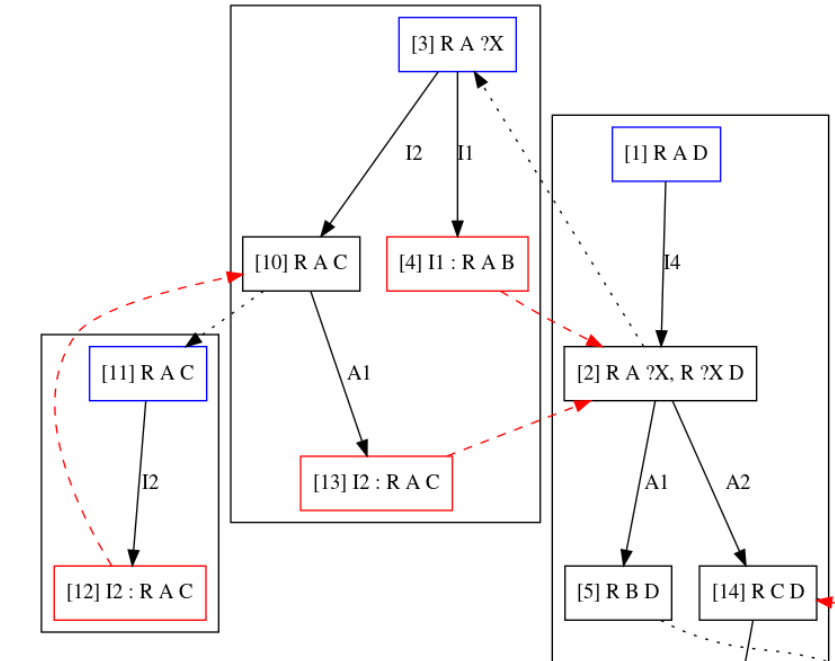
\includegraphics[height=0.5\textheight]{resolv}
  \end{center}

  Guarantees termination if size of typeclass problems is bounded
\end{frame}

%\begin{frame}[fragile]{New typeclass resolution: benefits for users}
%  \begin{itemize}
%  \item guarantees termination if size of typeclass problems is bounded
%  \item no need for transitive helper classes such as \texttt{HasCoeT}
%  \item \texttt{HasCoe a b} and \texttt{HasCoe b a} are simultaneously permissible
%  \end{itemize}
%  \bigskip
%
%\begin{leancode}
%instance coeTrans {α β γ : Type} [HasCoe β γ] [HasCoe α β] : HasCoe α γ
%instance coeBoolToProp : HasCoe Bool Prop
%instance coeDecidableToBool (p : Prop) [Decidable p] : HasCoe
%instance coeSubtype {α : Type} {p : α → Prop} : HasCoe {x // p x} α
%\end{leancode}
%\end{frame}

\begin{frame}[fragile]{State of the ⋃}
  \begin{onlyenv}<+-+(1)>
\begin{leancode}
notation "⋃ " binders ", " r:(scoped f, Union f) := r
\end{leancode}
    \vspace{-5mm}
    \begin{onlyenv}<+>
\begin{leancode}
expected ':='
\end{leancode}
    \end{onlyenv}
  \end{onlyenv}
  \begin{onlyenv}<+>
\begin{leancode}
notation "⋃ " b ", " r := Union (fun b => r)


#check ⋃ x,              x = x
#check ⋃ (x : Set Unit), x = x
#check ⋃ x ∈ univ,       x = x   -- error
\end{leancode}
  \end{onlyenv}
  \begin{onlyenv}<+>
\begin{leancode}
notation "⋃ " b ", " r := Union {b | r}


#check ⋃ x,              x = x
#check ⋃ (x : Set Unit), x = x
#check ⋃ x ∈ univ,       x = x   -- works!
\end{leancode}
  \end{onlyenv}
  \begin{onlyenv}<+-+(1)>
\begin{leancode}
syntax "⋃ " term ", " term : term
macro `(⋃ $b, $r) => `(Union {$b | $r})

#check ⋃ x,              x = x
#check ⋃ (x : Set Unit), x = x
#check ⋃ x ∈ univ,       x = x   -- works!
\end{leancode}
    \vspace{-5mm}
    \begin{onlyenv}<+>
\begin{leancode*}{stripnl=false}



syntax "{" term " | " term "}" : term
macro
| `({$x ∈ $s | $p}) => `(setOf (fun $x => $x ∈ $s ∧ $p))
| `({$x ≤ $e | $p}) => `(setOf (fun $x => $x ≤ $e ∧ $p))

| `({$b      | $r}) => `(setOf (fun $b => $r))
\end{leancode*}
    \end{onlyenv}
  \end{onlyenv}
  \begin{onlyenv}<+>
\begin{leancode}
syntax "⋃ " setIdx ", " term : term
macro `(⋃ $b, $r) => `(Union {$b | $r})

#check ⋃ x,              x = x
#check ⋃ x : Set Unit,   x = x  -- works!
#check ⋃ x ∈ univ,       x = x
\end{leancode}
    \vspace{-5mm}
\begin{leancode*}{stripnl=false}



syntax "{" term " | " term "}" : term
macro
| `({$x ∈ $s | $p}) => `(setOf (fun $x => $x ∈ $s ∧ $p))
| `({$x ≤ $e | $p}) => `(setOf (fun $x => $x ≤ $e ∧ $p))

| `({$b      | $r}) => `(setOf (fun $b => $r))
\end{leancode*}
  \end{onlyenv}
  \begin{onlyenv}<+>
\begin{leancode}
syntax "⋃ " setIdx ", " term : term
macro `(⋃ $b, $r) => `(Union {$b | $r})

#check ⋃ x,              x = x
#check ⋃ x : Set Unit,   x = x  -- works!
#check ⋃ x ∈ univ,       x = x
\end{leancode}
    \vspace{-5mm}
\begin{leancode}
declare_syntax_cat setIdx
syntax term                      : setIdx
syntax ident " : " term          : setIdx
syntax "{" setIdx " | " term "}" : term
macro
| `({$x ∈ $s | $p}) => `(setOf (fun $x => $x ∈ $s ∧ $p))
| `({$x ≤ $e | $p}) => `(setOf (fun $x => $x ≤ $e ∧ $p))
| `({$x : $t | $r}) => `(setOf (fun ($x : $t) => $r))
| `({$b      | $r}) => `(setOf (fun $b => $r))
\end{leancode}
  \end{onlyenv}
\end{frame}

%\newcommand{\status}[1]{\small\color{gray}[#1]}
%
%\begin{frame}[fragile]{New parser \status{mostly implemented}}
%  \begin{itemize}
%  \item completely accessible and extensible
%    \begin{onlyenv}<1>
%\begin{leancode*}{highlightlines={6}}
%@[parser]
%def my_inductive.parser : command_parser :=
%node! my_inductive ["inductive",
%  name: ident_univ_params.parser,
%  sig: opt_decl_sig.parser,
%  ext: node! my_inductive_base ["extends", base: term.parser]?,
%  local_notation: notation_like.parser?,
%  intro_rules: intro_rule.parser*]
%\end{leancode*}
%    \end{onlyenv}
%    \pause
%  \item arbitrary local backtracking and tokenizing
%    \begin{onlyenv}<2>
%\begin{leancode}
%notation `{` xs:(foldr `, ` (x xs, set.insert x xs) ∅ `}`)      := xs
%notation `{` binder ` // ` r:(scoped p, subtype p) `}`)         := r
%notation `{` binder ` ∈ ` s ` | ` r:(scoped p, set.sep p s) `}` := r
%\end{leancode}
%
%\begin{leancode}
%def symbol_quote.parser : term_parser :=
%node! symbol_quote [
%  left_quote: raw_str "`",
%  symbol: raw $ take_until (= '`'),
%  right_quote: raw_str "`" tt, -- consume trailing ws
%  prec: precedence.parser?]
%\end{leancode}
%      \vspace{-3cm}
%    \end{onlyenv}
%    \pause
%  \item concrete syntax tree fully accessible to tooling
%    \begin{onlyenv}<3>
%      \begin{itemize}
%      \item auto completion, document generation, code formatting, refactoring,
%        ...
%      \item jump to definition \emph{and documentation} of any syntax
%      \end{itemize}
%    \end{onlyenv}
%  \end{itemize}
%\end{frame}
%
%\begin{frame}[fragile]{Macros \status{mostly implemented?}}
%  \begin{itemize}
%    \item most general syntax sugars: arbitrary syntax tree transformations
%      \begin{onlyenv}<+>
%\begin{leancode}
%@[parser]
%def set_lit.parser : term_parser :=
%node! set_lit ["{", elems: sep_by ", " term.parser, "}"]
%
%@[transformer]
%def set_lit.transformer : transformer :=
%λ stx,
%  let v := view set_lit stx in
%  pure $ v.elems.foldr (λ x xs, `(set.insert %%x %%xs)) `(∅)
%\end{leancode}
%      \end{onlyenv}
%      \begin{onlyenv}<2>
%\begin{leancode}
%syntax set_lit := `{` (sep_by ", " term.parser) `}`
%
%syntax_translations set_lit
%| {}             := ∅
%| {%%x, %%xs...} := set.insert %%x {%%xs...}
%\end{leancode}
%
%        \raggedleft\emph{\color{gray}(hypothetical Isabelle-like macro-macros)}
%
%      \end{onlyenv}
%      \pause
%      \begin{onlyenv}<3>
%\begin{leancode}
%def my_inductive.transformer : transformer :=
%λ stx,
%  let v := view my_inductive stx in
%  pure $ review «inductive» {v with
%    intro_rules := match v.ext with
%    | some ext := {name := `base, sig := {params := [⟨`a, ext.base⟩]}} :: v.intro_rules
%    | none     := v.intro_rules
%  }
%end
%\end{leancode}
%      \end{onlyenv}
%      \pause
%    \item names are resolved (hygienically) only after expansion
%      \begin{onlyenv}<+>
%\begin{leancode}
%@[parser]
%def subty.parser : term_parser :=
%node! subty ["{", x: binder.parser, " // ", cond: term.parser, "}"]
%
%@[transformer]
%def subtype.transformer : transformer :=
%λ stx,
%  let v := view subty stx in
%  pure `(subtype (λ %%v.x, %%v.cond))
%\end{leancode}
%  %pure $ `(subtype %%(review lambda {binders := [v.x], body := v.cond}))
%      \end{onlyenv}
%      \begin{onlyenv}<+>
%\begin{leancode}
%syntax subty := `{` binder.parser ` // ` term.parser `}`
%
%syntax_translations subty
%| {%%x // %%cond} := subtype (λ %%x, %%cond)
%\end{leancode}
%  %pure $ `(subtype %%(review lambda {binders := [v.x], body := v.cond}))
%      \end{onlyenv}
%  \end{itemize}
%\end{frame}
%
%\begin{frame}[fragile]{Managing syntax \status{planned}}
%%  How do I replace the built-in \lean{inductive} command with my own?
%%  \pause
%%
%%\begin{leancode}
%%local attribute [-parser] lean.parser.inductive
%%local attribute [-parser] lean.parser.inductive
%%\end{leancode}
%
%  ``How do I manage my domain-specific set of notations?''
%
%  \pause
%  \begin{onlyenv}<2>
%\begin{leancode}
%namespace my_domain
%  -- @[parser]
%  def my_notation1.parser : term_parser := ...
%  ...
%end my_domain
%...
%local attribute [parser] my_domain.my_notation1
%local attribute [parser] my_domain.my_notation2
%local attribute [parser] my_domain.my_notation3
%...
%\end{leancode}
%
%    Hardly scalable...
%  \end{onlyenv}%
%  \pause%
%\begin{leancode}
%namespace my_domain
%  @[parser]  -- scoped by default
%  def my_notation.parser : term_parser := ...
%  ...
%end my_domain
%...
%open [parser] my_domain
%...
%\end{leancode}
%
%  Lean 2's scoped attributes return!
%  \pause
%
%  Main lesson we learned from Lean 2:
%
%  \emph{Most} attributes, like \lean{[reducible]} and \lean{[simp]}, should
%  \emph{not} be scoped (by default)
%\end{frame}
%
%\begin{frame}{Better trace logs \status{planned}}
%  make traces structured and lazy
%
%  \bigskip
%
%  \begin{minipage}{0.4\linewidth}
%    \begin{itemize}
%    \item collect trace points during initial elaboration
%      \uncover<2>{
%      \item when full trace is requested, re-elaborate
%        }
%    \end{itemize}
%    \vfill
%  \end{minipage}%
%  \begin{minipage}{0.6\linewidth} 
%    \begin{center}
%      \begin{onlyenv}<1> 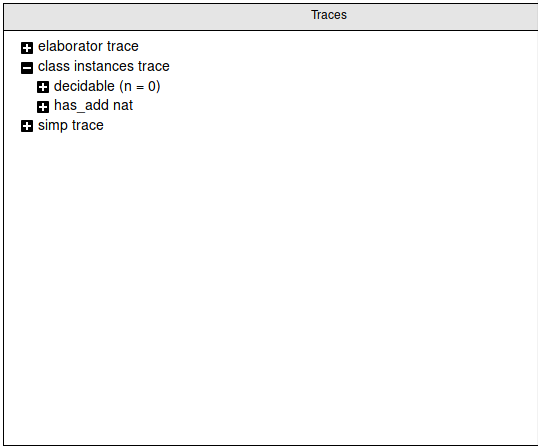
\includegraphics[width=0.9\textwidth]{traces}
%      \end{onlyenv}%
%      \begin{onlyenv}<2> 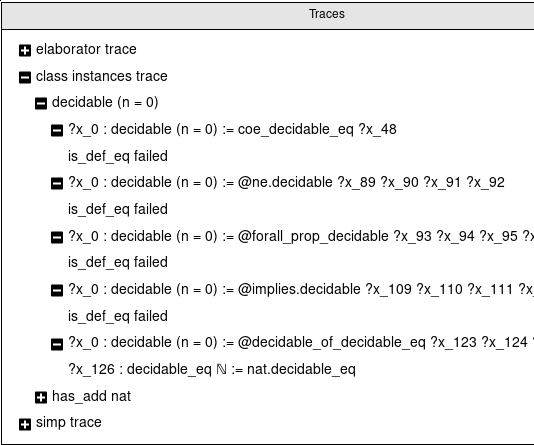
\includegraphics[width=0.9\textwidth]{traces_full}
%      \end{onlyenv}
%    \end{center}
%  \end{minipage}
%\end{frame}
%
%\begin{frame}[fragile]{More consistent namespacing \status{in progress}}
%  \begin{itemize}
%  \item \lean{open} is now ``sticky''
%\begin{leancode}
%open nat
%namespace nat
%  def random := 0
%end nat
%#check random
%\end{leancode}
%    \pause
%  \item \lean{parameters} have been removed to simplify resolution\footnote{\url{https://github.com/coq/coq/issues/6254\#issuecomment-450641538}}
%  \end{itemize}
%\end{frame}
%
%\begin{frame}[fragile]{Clarifying imports \status{proposal}}
%\begin{leancode}
%import init.data.set
%import data.set  -- ?
%
%open set  -- ??
%
%import ...two_dirs_up
%\end{leancode}
%  Connection between modules, packages, and namespaces in Lean 3 is not very clear
%  \pause
%
%  Proposal: Prefix module name with package name, use syntax more reminiscent of
%  file paths
%
%\begin{leancode}
%import "init/data/set"
%import "mathlib/data/set"
%
%open set
%
%import "../../two_dirs_up"
%\end{leancode}
%\end{frame}
%
\begin{frame}[fragile]{Thoughts about eventual porting of Lean 3 code}
  \begin{itemize}
  \item syntax changes: mostly superficial, automatable
    \pause

    One possible path: Incrementally reimplement Lean 3 syntax as macros first, then unfold
    them as final step
\begin{minted}{bash}
$ lean --plugin lean3-compat mathlib/src/...
\end{minted}
    \pause
  \item elaborator changes: probably not too drastic
    \pause
  \item library changes: mostly \emph{missing} API, needs to be reimplemented
    \begin{itemize}
    \item but not necessarily in the stdlib
    \end{itemize}
  \end{itemize}
\end{frame}
%
%\begin{frame}[fragile]{Conclusion}
%  \begin{itemize}
%  \item Many core features are starting to take shape
%  \item Still much to be done
%  \item Eventually should have many opportunities for community to get us back to
%    and beyond Lean 3's library
%  \end{itemize}
%
%  \pause
%  \vfill
%
%  \begin{onlyenv}<2> 
%  \begin{center}
%    \Huge{Thank you!}
%  \end{center}
%  \end{onlyenv}
%  \begin{onlyenv}<3> More presentations about Lean 4:
%    \begin{description}
%    \item[2018/08/03]
%      \href{http://leanprover.github.io/talks/LeanAtGalois.pdf}{\color{blue}\underline{Lean:
%          past, present and future}} by Leo
%    \item[2018/10/12] My
%      \href{http://leanprover.github.io/presentations/20181012_MSR}{\color{blue}\underline{internship
%          report}} - new parser, mostly
%    \item[2018/12/12]
%      \href{https://www.youtube.com/watch?v=Bv0CXyhbJ5s}{\color{blue}\underline{An
%          optimized memory model for an interactive theorem prover}}
%    \end{description}
%
%    \bigskip
%
%    Find these and more at
%    \begin{center}
%      \url{https://leanprover.github.io/publications}
%    \end{center}
%  \end{onlyenv}
%\end{frame}
\end{document}

%%% Local Variables:
%%% mode: latex
%%% TeX-master: t
%%% TeX-engine: luatex
%%% TeX-command-extra-options: "-shell-escape"
%%% End:
